\part{Fondements des expérimentations}

\chapter{Les défis du corpus}

\section{Les implications du corpus en méthodes quantitatives}

La constitution d'un corpus est fondamentale dans les études littéraires computationnelles. C'est à la fois sa grande force, car son caractère massif justifie l'utilisation de méthode quantitatives et sa plus grande faiblesse, puisque c'est le moment critique où les biais rentrent en compte et peuvent fausser les calculs et les résultats de l'étude. 

Dans un premier temps, il est important de préciser que le corpus ne vise pas à l'exhaustivité des textes écrits et publiés. Cela est simplement impossible, et l'idée est de prendre la fenêtre la plus large possible, pour représenter la majorité des courants et sous-genres littéraires. Nous visons un échantillon représentatif de ce qu'a pu être la production littéraire à une certaine époque. Bien que cette représentativité soit un idéal hors de portée, il faut tendre vers cet objectif. 

Comme nous l'avons dit, un des risques majeurs réside dans la constitution de biais qui fausseront l'ambition initiale de production de savoirs empiriques en histoire de la littérature. En effet, les biais sont des distorsions, des déformations systématiques d'un échantillon statistique, en l'occurrence un corpus de textes. Cela peut se caractériser par exemple par des biais temporels, qui focaliseront l'étude sur un grand nombre de textes d'une période donnée en minimisant l'importance d'autres périodes littéraires. 

De plus, si l'on veut étudier les pratiques littéraires génériques d'une période donnée, on ne peut pas se restreindre à un choix d'un petit nombre d'auteurs canoniques. Ce mémoire veut mettre au jour la présence de normes dans les pratiques stylistiques du canon littéraire. Si notre corpus contient une présence trop importante d'un sous-genre littéraire, par exemple le roman policier - réputé non-canonique - alors il est probable que l'on détecte non pas une norme générique, mais un ensemble de traits stylistiques propres à ce sous-genre précis. 

Il nous faut donc un corpus équilibré, autant dans le temps, que dans les sous-genres littéraires représentés. Enfin, il nous faut décrire rigoureusement le corpus sur lequel les analyses sont réalisées pour vérifier l'absence de biais, ou pour le moins en avoir conscience lors de l'analyse et de l'interprétation des résultats. 

\section{Le corpus d'étude}

Une des chances de cette présente étude est qu'elle arrive après une première salve de fouille de texte à grande échelle, dont une des missions principales était justement la constitution de grands ensembles de textes.    

Le projet \enquote{ANR Chapitres}\footnote{https://chapitres.hypotheses.org/} a recueilli un corpus massif de près de 3000 textes littéraires. Ce corpus est structuré en XML (eXtended Markup Language) avec un encodage TEI (Text Encoding Initiative), ce qui permet d'ajouter des méta-données aux textes, tels que le titre, l'auteur, l'éditeur, la date de parution ou encore le sous-genre romanesque. Nous mettons en annexe \ref{chapitre} la présentation de cette ANR. La période concernée s'étend sur deux siècles de production romanesque, du XIX\ieme au XX\ieme  siècle, comme on peut le voir en figure \ref{corpus_bar}. 

\bigskip
\begin{figure}[!ht]
    \centering
    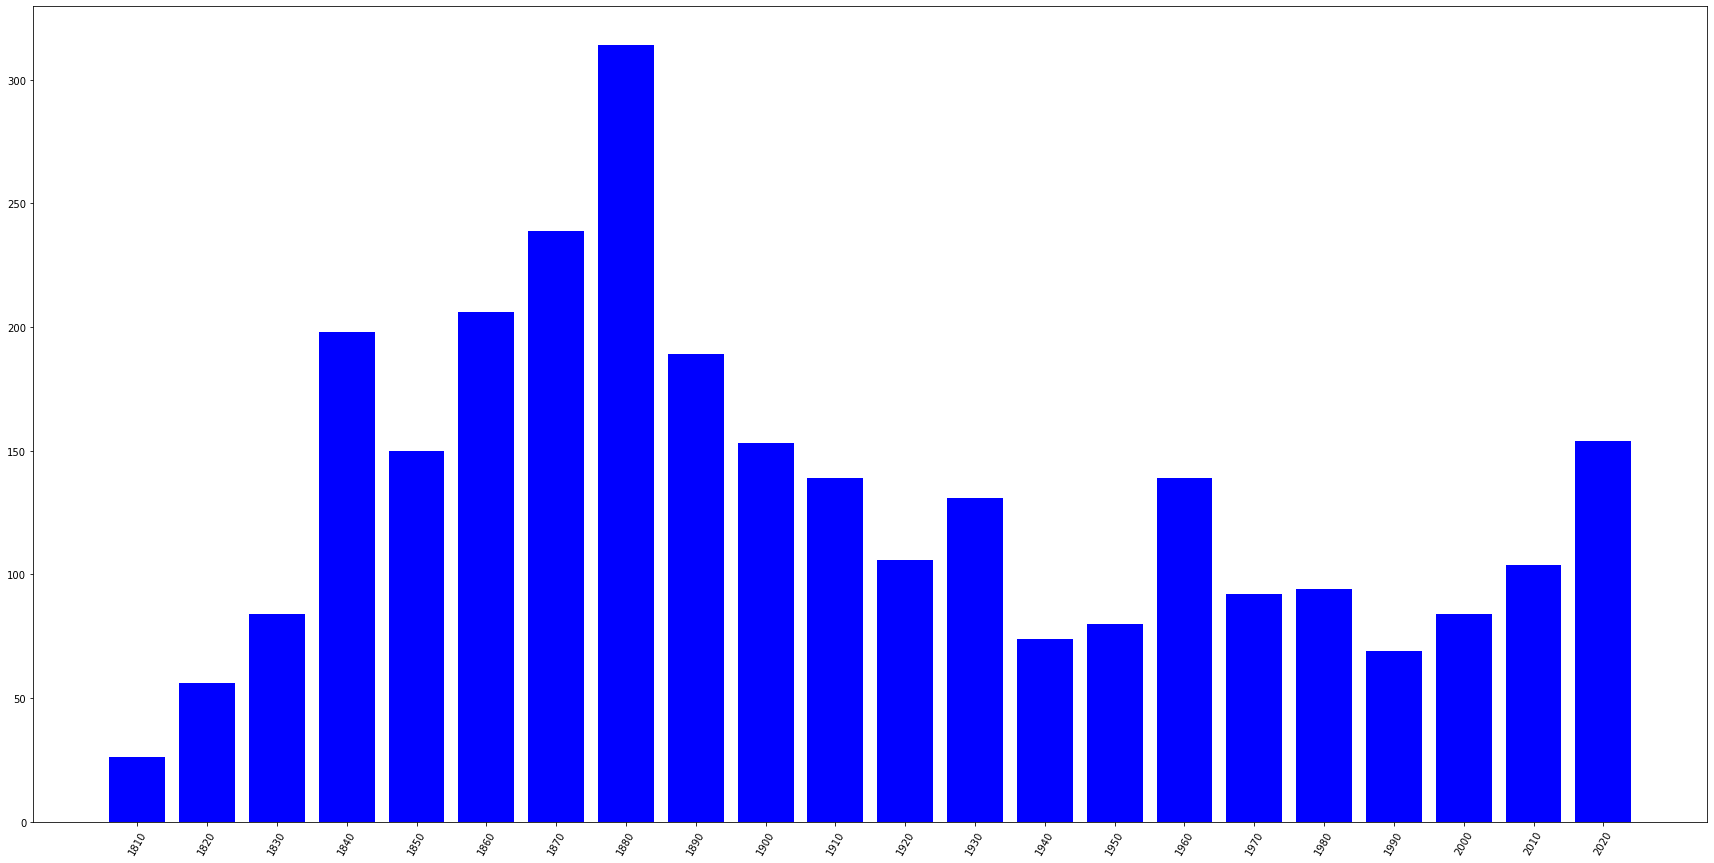
\includegraphics[width=15cm]{img/01_decades.png}
    \caption{Répartition du corpus dans le temps}
    \label{corpus_bar}
\end{figure}

La répartition dans le temps des romans de notre corpus est plutôt bonne, avec cependant la deuxième parie du XIX\ieme siècle qui comporte près de 40\% des romans. La décennie 1880 représente à elle seule près de 10\% des romans. Il faudra tenir compte de ces biais potentiels dans nos analyses, le risque étant de sur-représenter cette période dans les mesures statistiques. 

Le tableau \ref{Tab:statscorpus} décrit le corpus avec des statistiques simples. 

\begin{table}[ht]
\caption{Statistiques du corpus}
\centering
\bigskip
\begin{tabular}{lc}
    \hline
    Romans &  2953 \\
    Phrases &  14.982.817 \\
    Mots &  234.175.471 \\
    Moyenne de mots par roman & 79301 \\
    \hline
\end{tabular}
 \label{Tab:statscorpus}
\end{table}
\bigskip

L'un des biais principaux de ce corpus est qu'il rassemble les œuvres romanesques numérisées et disponibles sur internet. Cela implique nécessairement que ces textes ont été sélectionnés, publiés et conservés dans le temps, ce qui représente une partie infime de la production d'écrits. 

Pourtant, nous pensons que les ouvrages non-canoniques du corpus représentent un bon échantillon de ce qu'à pu être la production littéraire populaire, de par leur nombre - plus des 9/10 (cela dépend du critère que nous choisissons, nous verrons cela au prochain chapitre), mais aussi par la diversité des sous-genres représentés. La figure \ref{genres_corpus} montre les différents sous-genres du corpus, qui vont des romans policiers aux romans d'aventures, en passant par la science fiction. Il est important de noter que 2/3 des romans ont une étiquette de genre littéraire, ce qui représente selon nous un échantillon représentatif. Nous commenterons la répartition du canon dans le corpus en section \ref{notre_canon}.

\bigskip
\begin{figure}[!ht]
    \centering
    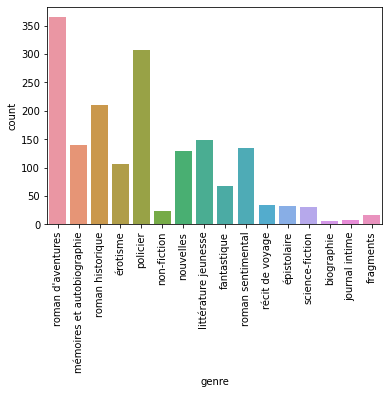
\includegraphics[width=15cm]{img/02_genres_corpus.png}
    \caption{Sous-genres littéraires du corpus}
    \label{genres_corpus}
\end{figure}



\chapter{Caractériser un canon littéraire}

\section{Méta-données : Enrichir le corpus}

Une des tâches principales du mémoire a été la construction d'un canon littéraire. Pour cela, nous entreprenons d'enrichir notre corpus avec les éléments de la réception actuelle des textes et des auteurs. Le canon littéraire n'est ni monolithique ni temporellement stable, le définir par des critères finis est en soi réducteur et néglige la complexité du phénomène. Mais nous allons essayer de nous focaliser sur des éléments déjà discutés et analysés par la critique littéraire et les études réalisées sur ce sujet. Un des aspects sur lequel nous allons nous concentrer est le rôle des institutions dans la formation du prestige littéraire. En premier lieu, tout le travail réalisé par Martine Jey et Laetitia Perret\footcites{jey_idee_2019} sur le rôle de l'institution scolaire dans la constitution de tels ensembles est prépondérant. Toutes deux ont montré que l'enseignement secondaire et supérieur avaient un impact énorme sur les processus de canonisation (dans la fabrication et surtout la conservation de ce canon) des auteurs et des textes. 


Travailler sur le canon littéraire à partir de la réception réalisée par les institutions scolaires nous paraît pertinent parce que cela s'inscrit dans une approche déjà éprouvée, bien qu'elle soit non exhaustive. En effet, d'autres facteurs entrent en jeu dans la constitution du canon, que ce soient des critères politiques, économiques ou sociologiques.

Il est important de noter que nous allons analyser la réception du canon littéraire par la réception actuelle, ce qui constitue aussi un élément discutable, mais la disponibilité des sources des méta-données (grâce à leur format numérique), nous a permis de recueillir énormément de données dans un temps réduit. 

Ainsi, nous avons établi un ensemble de critères non exhaustifs pour caractériser le canon littéraire que nous allons investiguer quantitativement.

\subsection{Le canon scolaire}

En premier lieu, nous nous sommes intéressés aux listes et au programmes des examens du secondaire, c'est à dire le brevet et le baccalauréat. Si l'on considère l'école républicaine comme le lieu de diffusion et de conservation du canon littéraire, alors il nous semble important de prendre en compte ce que l'on attend d'un élève lorsqu'il sort de l'enseignement obligatoire, c'est à dire ce qui constitue, pour les auteurs de ces listes, la culture littéraire minimale à la construction citoyenne. Le travail de Martine Jey, \enquote{La littérature au lycée : invention d’une discipline (1880-1925)}\footcites{jey_litterature_1998} décrit avec précision la construction d'une discipline, la littérature autour de textes garants d'une certaine langue et d'une certaine morale, qu'il faut diffuser pour éduquer les masses. Elle y analyse le processus d'intégration des œuvres dans le corpus scolaire qui est de fait un processus de canonisation. Au sein de l'enseignement scolaire et supérieur, les études littéraires produisent des formes distinctes de connaissances linguistiques\footnote{John Guillory, \enquote{Canon} in \cite{lentricchia_critical_2012},  p.43}. Il faudra donc récupérer des méta-données sur ces institutions qui construisent le canon littéraire.

%L'école fonctionne comme une institution sociale qui reproduit la structure stratifiée de l'ordre social.

\subsection{Le canon de l'enseignement du supérieur}

Dans un deuxième temps, nous nous sommes intéressés aux concours de l'enseignement du supérieur, qui incarnent le même rôle que précédemment mais avec un degré de prestige plus important. Nous avons récupéré les listes et les programmes de concours du supérieur (classes préparatoires littéraires et scientifiques du concours de l'ENS). Il s'agit d'évaluer et de sélectionner sur des connaissances littéraires, des candidats qui deviendront de futurs professeurs de collège. Michel P. Schmitt\footcites{schmitt_les_1993} a réalisé une démarche similaire en tenant des listes du nombre d'occurrences de citation d'auteurs dans les dissertations au CAPES interne. Sans passer par l'intérieur des copies, nous nous intéressons plutôt aux programmes des concours cités.

\subsection{Le canon des concours de l'agrégation}

Nous avons également récupéré les programmes des concours des agrégations de lettres modernes, plus haut concours de recrutement dans la fonction publique pour des professeurs. Il nous semblait significatif de constater quels étaient les auteurs et les textes sur lesquels on formait l'élite des professeurs de lettres de la République. Pour un panorama des épreuves de l'agrégation, les recherches de Martine Jey\footcites{jey_canon_2014}, d'André Chervel\footcites{chervel_histoire_1993} et de Yves Chevrel\footcites{chevrel_les_2003} ont été d'une grande aide.
Comme ces programmes ne comportaient pas beaucoup de romans, nous avons décidé d'agrandir la période de réception considérée. Pour cette méta-donnée précisément, nous remontons jusqu'en 1950.  

\subsection{Le canon des éditeurs}

Ensuite, nous nous sommes intéressés au monde de l'édition, qui est aussi un des acteurs majeurs dans le processus de canonisation des oeuvres. La thèse de Dragos Jipa\footcites{jipa_canonisation_2016} a bien montré, avec la collection des \enquote{Grands écrivains de France}, l'importance des logiques éditoriales dans la construction d'un consensus national autour d'un panthéon d'auteurs. 

Nous nous sommes intéressés à la collection de la Pléiade qui est l'exemple typique du rôle des éditeurs dans la canonisation d'auteurs. La publication des écrits d'un auteur en oeuvres complètes vient souvent parachever une carrière littéraire, souvent après la mort de l'auteur. Elle est un signe majeur dans la reconnaissance du-dit auteur en tant qu'appartenant au canon littéraire. C'est aussi une des portes privilégiées pour les éditeurs car elle permet de sacraliser de nouvelles têtes et d'en tirer profit par effet de levier. La collection de la Pléiade comporte finalement peu d'auteurs de romans, et consacre un auteur dans sa totalité. Malgré tout, nous récupérons tous les auteurs publiés dans la Pléiade.

% Quelle couverture XX vs XIX ème siècle ?
%+gné avant

Pour plus de finesse, nous prenons également l'édition Garnier-Flammarion et plus précisément la collection \enquote{littérature et civilisation}. Un des traits majeurs de cette collection est qu'elle présente les romans avec un appareil critique qui accompagne la lecture de l'ouvrage. Cet appareil critique n'est pas anodin et montre que l'ouvrage a une portée qui requiert explication. Le canon littéraire est rempli d'oeuvres qui valent la peine que l'on se penche sur elles et leur contextes. Cela nous intéresse parce que cette vision pédagogique du canon littéraire est très répandue et est même un des arguments au statu-quo littéraire en France et ailleurs\footcites{guillory_cultural_1998}.  

\subsection{Le canon de la critique}
Pour prendre un témoin de la critique littéraire, nous nous sommes intéressés aux prix littéraires. Ces derniers constituent la partie de notre canon la moins résistante au temps, car ils sont embourbés dans des dimensions économiques et politiques très fortes comme l'a résumé James F. English dans son livre sur la circulation de la valeur culturelle\footcites{english_economy_2009}. Malgré ces remarques, nous voulions mesurer son effet dans les pratiques littéraires. Ainsi nous avons récupéré les listes des prix littéraires les plus importants, du prix Goncourt au prix Femina. 

Enfin nous prenons en compte la recherche contemporaine, avec une canonicité à l'échelle de l'auteur et la revue littéraire en ligne \enquote{Fabula\footnote{https://www.fabula.org/}}. Cet aspect était déjà présent dans les méta-données du corpus Chapitres (voir en annexe \ref{chapitre}), et nous avons décidé de le conserver. 

\section{Notre canon}\label{notre_canon}

Ainsi construit avec plusieurs facteurs, notre canon littéraire se trouve moins discutable puisqu'il cherche à multiplier les entrées dans les différents acteurs du champ littéraire qui définissent, nourrissent et conservent le canon littéraire. 

Une grande partie de ces données, notamment celles du brevet et du baccalauréat ont été récupérées grâce à l'immense travail du collectif \textit{Le deuxième texte}\footnote{https://george2etexte.wordpress.com/} qui a mis en ligne ses données\footnote{https://www.data.gouv.fr/fr/organizations/le-deuxieme-texte/} en open source. D'autres ont été récupérées automatiquement à l'aide de scripts python sur les pages web de la collection Garnier-Flammarion et de la Pléiade, mais aussi à la main pour les auteurs présents dans le Lagarde et Michard (Bordas) du XIX\ieme siècle et du XX\ieme siècle.

Nous avons décidé d'établir une double approche quand à l'appartenance ou non au canon littéraire. La canonicité revient d'une part à la granularité du roman, et d'autre part à celle de l'auteur. 

Nous construisons ainsi deux canons littéraires, à l'échelle des auteurs et des textes. Nous mettons en annexes les listes détaillées de ces deux ensembles, avec en annexe \ref{canon_auteur} la liste des auteurs canoniques, et en annexe \ref{canon_roman} la liste des romans canoniques, triée par année de première parution. L'échelle de l'auteur agrandit énormément le cercle, puisque toutes les oeuvres d'un auteur canonique sont considérées comme canoniques. Si l'approche la plus intéressante nous paraissait la première à l'échelle de l'œuvre, nous avons conservé les deux qui méritaient tout autant des tests approfondis. 

Pour faire correspondre notre corpus au canon construit par nos soins, il a été décidé de réaliser un simple test d'appartenance, si le titre d'un roman appartient à au moins une liste, le roman en question est considéré comme canonique. Même chose pour l'auteur, s'il est présent dans une des listes établies, tous les textes de l'auteur sont considérés comme canoniques. Ainsi, le nombre des ouvrages du corpus qui sont dans notre canon s'élève à 264 éléments (moins de 1\% du corpus), tandis que le nombre des œuvres dont les auteurs sont dans notre canon est de 1156 romans, soit 39\%.

Nous avons pensé mettre en place un indice de canonicité, pour mieux représenter la réalité du monde littéraire, qui n'est pas d'une binarité sans conditions, entre canon et non canon. Un auteur est plus ou moins canonique, et Honoré de Balzac l'est plus qu'Anatole France par exemple. Mais nous manquions de temps et de données pour présenter une telle approche, et après des essais peu fructueux, nous conservons notre test d'appartenance binaire.

Pour bien vérifier la viabilité de ces approches, nous avons réalisé des statistiques descriptives pour voir comment notre canon se comportait dans le corpus. 

\bigskip
\begin{figure}[!ht]
    \centering
    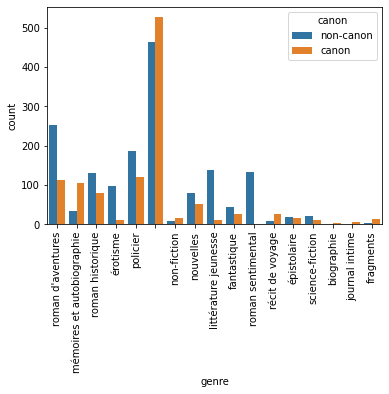
\includegraphics[width=15cm]{img/03_genres_corpus_canon.png}
    \caption{Répartition du canon dans les sous-genres du corpus}
    \label{genre_corpus_canon}
\end{figure}

On constate dans la figure \ref{genre_corpus_canon} une bonne répartition des oeuvres du canon des auteurs dans les sous-genres littéraires du corpus. Il faut souligner que les ouvrages canoniques sont de fait moins représentés que ceux canoniques, puisque le corpus en comporte seulement 39\%. La seule anomalie à constater est au sein des ouvrages non-étiquetés par un genre, où le canon est plus représenté que les non-canons. Mais la différence d'une cinquantaine d'ouvrages n'est pas énorme, et l'on ne peut pas conclure dans ce cas que le canon des romans n'est qu'un agrégat de sous-genres littéraires spécifiques.

\bigskip
\begin{figure}[!ht]
    \centering
    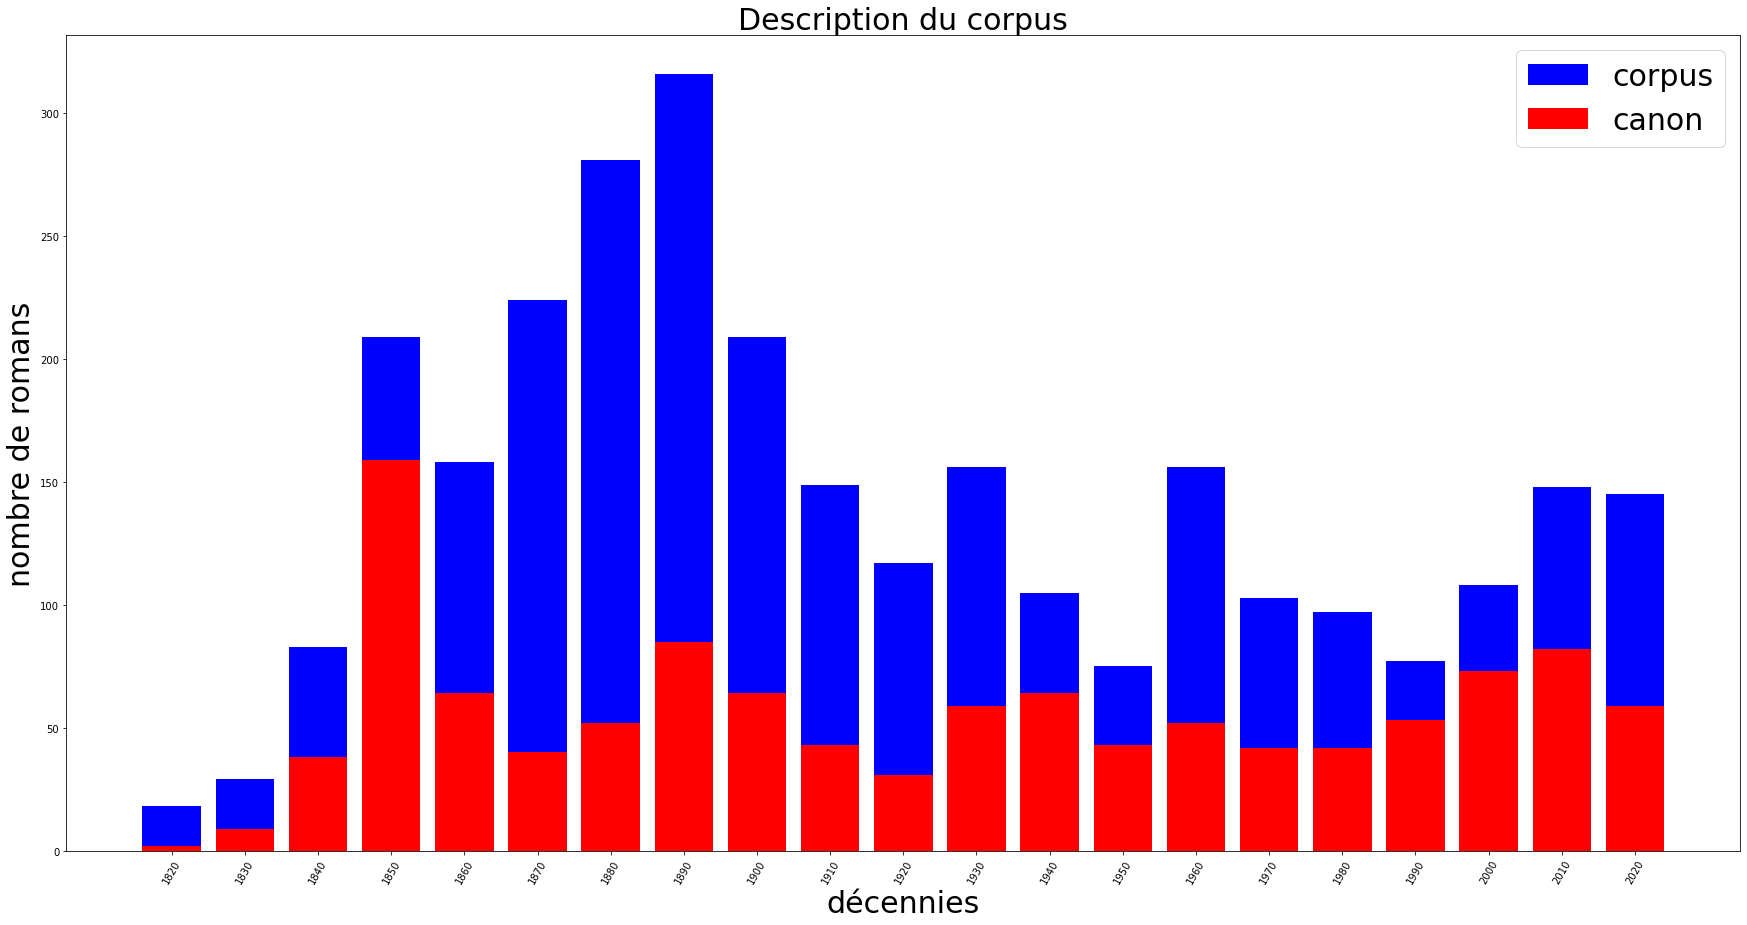
\includegraphics[width=15cm]{img/04_corpus_bar.png}
    \caption{Répartition du canon dans le temps}
    \label{corpus_bar_temps}
\end{figure}

La figure \ref{corpus_bar_temps} représente la présence de notre canon au fil de l'histoire littéraire. Il est assez bien réparti et suis l'évolution de la population du corpus. On remarque que la décennie de 1840 à 1850 comporte plus de canon que de non-canon, mais c'est la seule dans ce cas.

Ainsi, le genre littéraire ou la date de parution ne sont pas des facteurs définitifs pour expliquer la présence de romans ou d'auteurs dans le canon. Notre approche, qui est d'ouvrir les romans et de s'intéresser au contenu textuel de manière quantitative est justifié, dans le sens où le texte est un facteur qui pourrait contribuer à apporter des éléments de réponses. 


\chapter{Méthodes et outils}

Les méthodes du traitement automatique des langues sont d'une grande assistance. En plus de nous aider au pré-traitement et au nettoyage des textes, elles nous permettent de récupérer les caractéristiques textuelles sur lesquelles notre classification automatique se fonde. Nous présentons, dans les sections qui suivent, la méthode que nous mettons en place.

\section{Les données textuelles}

Nous voulons mettre au jour une esthétique canonique dans nos textes. On s'intéresse donc à des éléments formels, qui seraient des indices linguistiques issus de la filtration des textes jusqu'à la réception actuelle. Le phénomène que nous voulons modéliser est complexe, et pas évident puisque c'est un phénomène à réception, qui viendrait consacrer un texte ou un auteur après l'écriture de ses textes. Face à la complexité du phénomène que nous envisageons, nous avons voulu simplifier les caractéristiques textuelles retenues. En effet, le meilleur moyen de prendre en compte le contenu textuel de nos romans est de récupérer des informations sur les mots de ces derniers. Cette méthode a déjà été utilisée par des chercheurs déjà cités, notamment Ted Underwood dans son article \enquote{La longue durée du prestige littéraire}\footcites{underwood_longue_2016}.  Nous aurions pu prendre des éléments plus complexes, relatifs au style ou à la littérarité des ouvrages comme la longueur des phrases, l'avancée narrative ou les thèmes du récit. Mais la relation entre complexité du style, littérarité et prestige littéraire n'est pas si évidente que cela, et nous décidons d'une première approche \enquote{simple}, que l'on pourrait complexifier par la suite, si ces premières recherches se trouvaient fructueuses.

Ainsi nous décidons de transformer nos ouvrages en \textit{sac-de-mots}. Les textes sont ainsi décomposés en des listes de mots qui indexent leur fréquence relative (le nombre de fois où l'unité apparaît, divisé par la longueur totale du texte). Chaque unité est traitée comme une caractéristique des textes dans lesquels elle apparaît - une sorte de trait d'identification - et le texte devient un vecteur de ces traits. 

Nous décidons de limiter notre sac de mots au 1000 uni-grammes les plus fréquents récupérés dans un échantillon de 200 textes tirés au hasard dans le corpus.  Deux raisons à cela, une première pratique, puisque la prise en compte de tous les mots du corpus aurait nécessairement amené à des coûts computationnels très importants, car les matrices résultantes auraient été très éparses, avec beaucoup de fréquences d'apparitions nulles ou proches de zéro. La seconde raison réside dans la nature des mots que nous récupérons. Comme ce sont les mots les plus fréquents du corpus, la plupart sont des déterminants, prépositions et autres \textit{mots-outils}. Ces derniers relèvent plus d'une écriture inconsciente et automatique des auteurs qu'à des mots moins fréquents relatifs au contenu et aux thèmes du textes. Il ne nous semble pas que les mots de nature thématique jouent un rôle dans la spécificité des textes à être canoniques ou non. Cela nous permet également de ne pas prendre en compte une grande majorité des noms communs ou des noms propres, qui ne nous intéressent pas à cette échelle.

Ces \textit{mots-outils} sont au coeur de la stylométrie, notamment dans les attributions d'auteur\footcites{burrows_delta_2002}, et dans l'étude des idiolectes\footcites{seminck_evolution_2022}, c'est à dire de la signature textuelle d'un écrivain. Ces méthodes ont produit de très bons résultats, allant de Hildegarde de Bingen\footcites{kestemont_function_2014}, à Shakespeare\footcites{plechac_relative_2021} ou Molière\footcites{cafiero_why_2019} et Racine\footcites{cafiero2021psyche}. Si le problème auquel nous faisons face n'est pas de même nature, nous pensons que ces techniques sont pertinentes pour traiter notre problème. En effet, s'il y a bien une manière particulière de faire littérature selon les institutions qui forment le canon littéraire, alors nous devrions retrouver les marqueurs inconscients de cette sélection. 

Pour quantifier les fréquences d'apparition de mots, on réduit les unités lexicales sujettes à flexion (les verbes, les substantifs, les adjectifs) à leur unité lexicale commune. On appelle ce processus \textit{lemmatisation}. Pour ce traitement, nous utilisons la librairie Spacy. Elle nous permet de tokeniser, lemmatiser et de nettoyer les romans en contrôlant l'étiquetage morphosyntaxique des tokens. La figure \ref{work_flow} représente la chaîne de traitement de la récupération des données textuelles.

\bigskip
\begin{figure}[!ht]
    \centering
    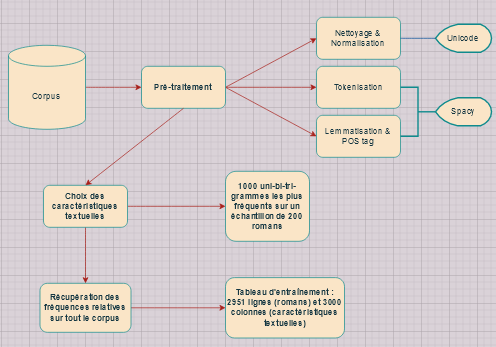
\includegraphics[width=15cm]{img/05_work_flow.png}
    \caption{Récupération des données textuelles : Flux de travail}
    \label{work_flow}
\end{figure}

Des recherches récentes en classification de textes littéraires ont montré que la prise en compte des contextes d'un mot pouvait avoir des impacts important sur les résultats d'une classification\footcites{van_cranenburgh_identifying_2015}. Ainsi, nous décidons de prendre en compte, en plus des uni-grammes, des bi-grammes et des tri-grammes de lemmes. Ces derniers sont agrégés par la concaténation de deux ou trois lemmes. Nous procédons de la même manière que pour les uni-grammes, en prenant les 1000 éléments les plus fréquents pour chaque type.

Finalement, nous obtenons un grand tableau de données, avec en colonnes les trois mille caractéristiques textuelles que l'on vient de définir, et en lignes chaque roman de notre corpus. Le tableau est rempli avec les fréquences relatives pour chaque caractéristique.  

\section{Outils de programmation}

Nous fondons notre travail sur le langage de programmation Python et les librairies construites au-dessus. Pour l'analyse des données et leur manipulation nous utilisons Pandas\footnote{https://pandas.pydata.org/} et Numpy\footnote{https://numpy.org/}. Pour le traitement du texte à proprement dit, nous employons la librairie Spacy\footnote{https://spacy.io/}. Cette dernière est très performante pour une analyse sur de grandes quantités de données et couvre tous les traitements d'une chaîne de TAL classique. Cette librairie est un peu moins performante pour le français des textes littéraires, parce qu'elle a été entraînée sur des contenus de presse récente. D'autres librairies proposent des modèles un peu plus performants, comme la librairie Stanza\footnote{https://github.com/stanfordnlp/stanza} ou Pie-Extended\footnote{https://github.com/hipster-philology/nlp-pie-taggers}. Pour autant, après des tests de ces différentes librairies, Spacy se montrait la plus efficace en terme de temps d'exécution, avec un nombre d'erreurs plus important que les deux autres mais relativement réduit dans l'ensemble. Avec nos moyens informatiques limités, nous avons privilégié cette librairie pour parser nos 3000 romans. Cette dernière a aussi l'avantage d'être très bien documentée et comporte plusieurs modèles de langages pour le français. Au vu des performances des différents modèles, nous prenons la décision d'utiliser le modèle fr\_core\_news\_lg qui a un très bon rapport d'utilisation de ressources temporelles et matérielles entre exécution et performance. Nous utilisons aussi Scikitlearn\footnote{https://scikit-learn.org/stable/index.html}, qui donne des outils efficaces pour l'analyse prédictive de données. Scikitlearn est assez simple à utiliser et implémente des algorithmes d'apprentissage machine au niveau de l'état de l'art.

\section{Modélisation statistique}

Nous voulons observer si des différences statistiques majeures existent entre nos deux sous-corpus, celui canonique et celui non-canonique. Nous faisons appel au champ de recherches de l'apprentissage machine. L'objectif de la modélisation statistique est de tirer des généralisations sur de grands jeux de données. Un exemple explicite est la régression linéaire, qui cherche à établir une relation entre des variables diverses. 

L'apprentissage machine fait référence à toute une série d'algorithmes statistiques qui traitent chaque texte comme un amalgame de certaines caractéristiques quantifiables. Cette approche part du principe que l'on peut quantifier leur répartition dans les textes de manière à identifier les différences entre ces derniers, afin de classifier ou prédire la catégorie à laquelle un texte est susceptible d'appartenir. 

%L'intérêt de l'apprentissage automatique est justement de modéliser des pratiques de catégorisation qui n'ont pas de définition et qui peuvent être déduites uniquement d'exemples. Nous ne savons peut-être pas comment décrire un spam, même si nous le reconnaissons dans notre boîte mail. Un filtre anti-spam commence donc par un apprentissage composé de messages que les lecteurs ont ou n'ont pas marqué comme spam. Un algorithme apprend à modéliser le spam en utilisant tous les détails textuels qui, en pratique, distinguent ces groupes de groupes de messages.

La classification automatique de textes est un problème très étudié en statistiques. Plusieurs estimateurs sont au niveau de l'état de l'art : des modèles linéaires, comme le naïve bayes ou la classification ridge. Une famille de modèle retient particulièrement notre attention parce qu'elle obtient de bons résultats pour la classification de textes littéraires: les Machines à Vecteur de Support (SVM)\footcites{yu_evaluation_2008}. Les SVM ont pour but de trouver les plans qui séparent les points de données avec les marges maximales entre les frontières de décision. Ils traitent les caractéristiques comme des coordonnées dans un espace cartésien à haute dimension et tentent de tracer une ligne qui divise au mieux les caractéristiques uniques d'une classe\footnote{Pour de plus amples informations sur les SVM, voir l'article fondateur de Vladimir Vapnik dans \cites{cortes_support-vector_1995}}. Pour l'estimateur SVM, un texte n'est qu'une combinaison de caractéristiques qui tendent à apparaître plus souvent dans une classe de textes que dans une autre. Le modèle assigne des coefficients à chaque mot pour estimer la probabilité que le roman soit canonique. 

Les SVM ont l'avantage de réduire le risque de sur-apprentissage. Ce dernier se caractérise lorsqu'un modèle statistique se spécialise trop sur ses données d'entraînement, ce qui réduit sa performance de généralisation. Nous utilisons dans ce mémoire la famille de SVM développé par l'équipe scikit-learn\footcites{scikit-learn_2011} depuis 2011.

Nous avons affaire à une approche très connue en apprentissage machine : l'apprentissage supervisé. Ce dernier est assez simple à comprendre, puisqu'il associe un ensemble de données avec une certaine classe labellisée. Un modèle statistique est évalué sur sa capacité à faires des inférences entre les particularités des données et une certaine classe. Les classes de nos romans correspondent aux méta-données récupérées, c'est à dire si le roman en question appartient ou non au canon littéraire.

\subsection{Implémentation de l'apprentissage machine}

Nous mettons en place les bases de l'apprentissage machine. Le jeu de données est séparée en deux échantillons. 

\begin{itemize}
    \item Un premier sur lequel nous entraînons le modèle statistique, c'est à dire que nous lui donnons le label associé pour chaque roman.
    \item Un autre sur lequel nous évaluons ses performances de prédictions sur des données qu'il n'a jamais vu. 
\end{itemize} 

Nous mesurons ainsi la capacité du modèle à généraliser.

Nous voudrions que la taille de l'échantillon du corpus d'entraînement soit la plus large possible, pour donner toutes ses chances au modèle. Pour autant, il est important de garder une taille conséquente pour l'échantillon de test afin de mesurer à quel point le modèle est capable de réaliser de bonnes prédictions sur un grand nombre de données. Nous fixons la taille de l'échantillon test à 20\% du total. 

Nous implémentons grâce à Scikitlearn un pipeline avec un pré-traitement des données, un StandardScaler et un estimateur, le SVM. Ce pré-traitement permet de normaliser nos données. La normalisation d'un ensemble de données est une exigence commune à de nombreux estimateurs d'apprentissage automatique : ils peuvent mal se comporter si la distribution statistique ne ressemble pas à des données distribuées sous forme d'une loi normale. Nous avons implémenté le SVM du logiciel SuperStyl\footcites{Camps_SUPERvised_STYLometry_SuperStyl_2021}, de Jean-Baptiste Camps, puis nous avons codé un algorithme mieux adapté à notre approche, avec des estimateurs plus performants et une méthode spécifique pour une classification binaire.\footnote{Voir en annexe \ref{code} le lien du github avec le code du mémoire} 

Nous contrôlons la robustesse de nos résultats par une validation croisée en cinq parties. Cette validation est une procédure qui permet d'éviter le sur-apprentissage et de garantir la fiabilité de nos modèles. Elle sépare l'ensemble du jeu de données en cinq parties, et réalise cinq entraînements distincts en prenant à chaque fois quatre parties pour l'entraînement et une pour s'évaluer. La moyenne de l'efficacité du modèle sur ces cinq entraînements est ainsi un score beaucoup plus robuste et fiable. 

\subsection{Métriques d'évaluation du modèle}

Nous évaluons notre modèle grâce à des métriques d'évaluation de la performance : l'efficacité, la précision, le rappel et un f1-score.

Pour comprendre ces métriques, il faut se familiariser avec les notions de vrai-positif (TP), vrai-négatif (TN), faux-positif (FP) et faux-négatif (FN). Dans notre cas, un TP est un roman considéré comme canonique par nos méta-données et prédit comme tel. Un TN est un roman non-canonique prédit comme non-canonique. Un FP est un roman non-canonique prédit comme canonique. Un FN est un roman canonique prédit comme non canonique. Une prédiction sans erreur équivaut donc à minimiser les mauvaises attributions, c'est à dire minimiser FP et FN. 

L'efficacité est la métrique la plus simple à comprendre, puisque c'est le pourcentage d'éléments prédits correctement par le modèle. 

\begin{equation}
Efficacite = \frac{TP + TN}{TP + TN + FP + FP}.
\end{equation}


\bigskip
\begin{figure}[!ht]
    \centering
    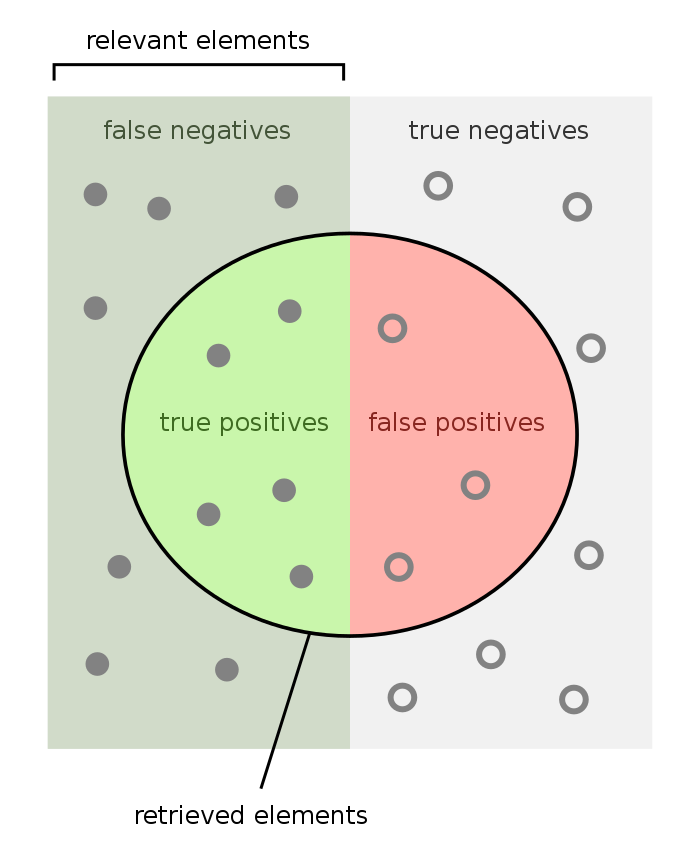
\includegraphics[width=10cm]{img/06_precision_recall.png}
    \caption[Précision et rappel 1/2]{Précision et rappel 1/2\footnotemark}
    \label{modelevaluation}
\end{figure}


Comme on peut le voir sur la figure \ref{modelevaluation}, la précision est la fraction d'éléments pertinents parmi les éléments extraits. Autrement dit, la précision est définie par : 

\begin{equation}
Precision = \frac{TP}{TP + FP}.
\end{equation}
 

Le rappel est la fraction d'éléments pertinents qui ont été extraits. Autrement dit, le rappel est définie par :
\begin{equation}
Rappel = \frac{TP}{TP + FN}.
\end{equation} 
\footnotetext{\textit{ Source : }$https://en.wikipedia.org/wiki/Precision\_and\_recall$}

\bigskip
\begin{figure}[!ht]
    \centering
    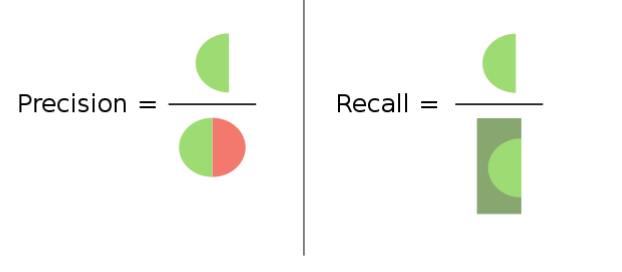
\includegraphics[width=10cm]{img/07_preci_recall.png}
    \caption[Précision et rappel 2/2]{Précision et rappel 2/2\footnotemark}
    \label{preci_recall}
\end{figure}

\footnotetext{\textit{ Source : }$https://en.wikipedia.org/wiki/Precision\_and\_recall$}

Le score F1 peut être interprété comme une moyenne harmonique de la précision et du rappel, où un score F1 atteint sa meilleure valeur à 1 et son pire score à 0. La formule pour le score F1 est la suivante : F1 = 2 * (précision * rappel) / (précision + rappel)

Il faut être attentif à ces trois métriques pour s'assurer de la viabilité du modèle et de sa performance. En effet, même lorsque l'efficacité du modèle est très bonne, les autres mesures peuvent, par exemple dans le cadre d'un jeu de données peu équilibré, montrer les limites du modèle en donnant des scores très bas.


Ainsi, nos expérimentations se fondent sur trois piliers principaux. Un corpus d'étude, un canon construit par nos soins et les méthodes quantitatives. A partir de cela, nous proposons de modéliser la notion de canon littéraire pour poser un diagnostique quantitatif de la filtration du contenu littéraire au cours du temps.